% Provenance (never printed): old premiere S material on magmatic rocks (volcanic
% and plutonic textures and cooling rate; basalt/gabbro, andesite/diorite,
% rhyolite/granite; order of crystallisation, told). Cooling of sheets from
% figdata/grade-11/dyke_cooling.py (Delaney 1986 parameters; kappa from England
% et al. 2007). Fractional crystallisation is Year 2's; metamorphism (contact
% aureoles) is g12.03's: not developed here.
\chapter{Stollingsgesteenten}\label{ch:g11:igneous-rocks}

Aan de noordkust van Ierland dalen stenen zuilen, dicht tegen elkaar, af
in de zee: de Giant's Causeway, een basalt dat
uit een lava is afgekoeld. In Yosemite, in Californië, rijst de granieten wand van El
Capitan zo'n \qty{900}{m} boven de dalbodem uit, één enkel lichaam van
grofkorrelig gesteente. Beide zijn uit magma gekristalliseerd. Het basalt koelde aan het
oppervlak af, met kristallen die te klein zijn om te zien; het graniet koelde diep onder de grond af,
met kristallen die groot genoeg zijn om te zien, en het is vandaag alleen zichtbaar omdat
de gesteenten erboven zijn weggesleten. Dit hoofdstuk leest in de korrels van een gesteente
hoe snel, en hoe diep, het is afgekoeld.
% ledger: photo:g11-giants-causeway, photo:g11-el-capitan, tulane:intrusions

\begin{omfigure}
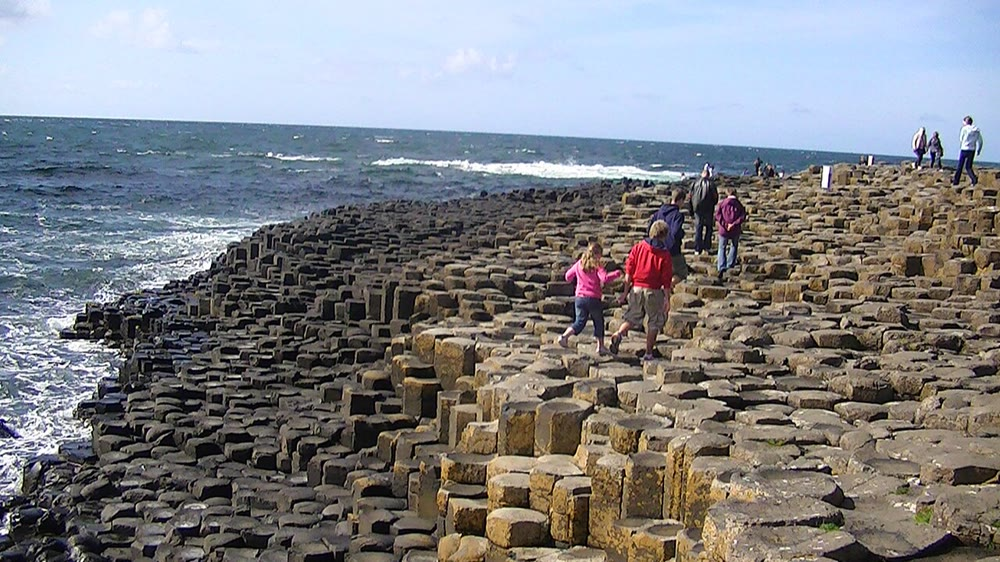
\includegraphics[height=4.3cm]{images/book2/g11-bishop-giants-causeway.jpg}\hspace{0.04\linewidth}%
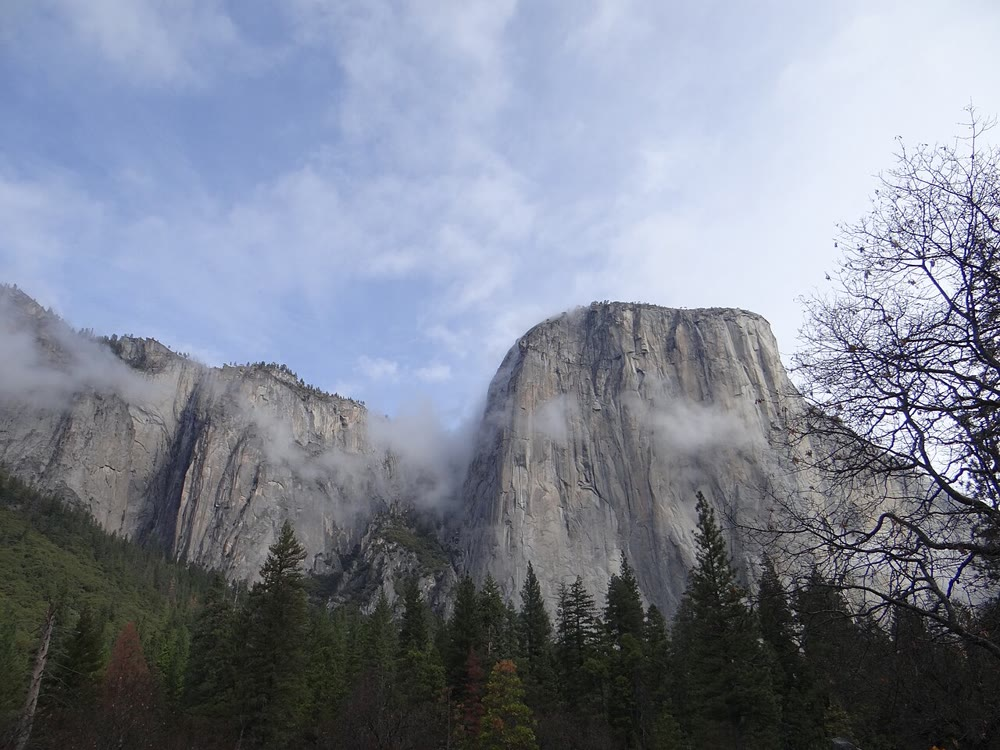
\includegraphics[height=4.3cm]{images/book2/g11-usgs-el-capitan.jpg}

{\small Links: basaltzuilen van de Giant's Causeway, Noord-Ierland.
Foto Adam Bishop (CC~BY-SA~3.0). Rechts: El Capitan, Yosemite,
Californië, een granietwand van ongeveer \qty{900}{m} hoog. Foto U.S.
Geological Survey (CC0).}
\end{omfigure}
% ledger: photo:g11-giants-causeway, photo:g11-el-capitan

\begin{recall}
Magma is gesmolten gesteente onder het oppervlak; het barst uit als lava, rustig of
explosief (Boek 1, jaar 7). Een stollingsgesteente ontstaat wanneer gesmolten
gesteente afkoelt en vast wordt (Boek 1, jaar 6). Basalt is een donker \omterm{def:g11:igneous-rocks:volcanic-plutonic}{vulkanisch gesteente}, graniet een
licht gesteente van veldspaat, kwarts en mica (Boek 1, jaar 6).
Mantelperidotiet smelt gedeeltelijk wanneer hij onder een rug opstijgt, en levert het basalt en
\omterm{def:g11:ocean-ridges:gabbro}{gabbro} van de \omterm{def:g11:ocean-ridges:oceanic-lithosphere}{oceanische korst} (\cref{ch:g11:ocean-ridges}). De \omterm{def:g11:minerals:rock-forming}{gesteentevormende
silicaten} zijn olivijn, pyroxenen, amfibolen, mica's, veldspaten en kwarts;
de veldspaten zijn kaliveldspaat en plagioklaas, een reeks van
calciumrijk tot natriumrijk (\cref{ch:g11:minerals}). Warmte verspreidt zich door
geleiding over een afstand van ongeveer $\sqrt{\kappa t}$ in een tijd $t$, waarbij
$\kappa$ de thermische diffusiviteit is (\cref{ch:g11:subduction-zones}).
\end{recall}
% ledger: tulane:ridge-rocks, england:kelvin

\section{Vulkanische en plutonische gesteenten}

\begin{definition}[Vulkanisch gesteente; plutonisch gesteente]\label{def:g11:igneous-rocks:volcanic-plutonic}
Een stollingsgesteente, gevormd door de kristallisatie van een magma, is
\emph{vulkanisch}\index{vulkanisch gesteente}
(of extrusief) wanneer het magma aan het aardoppervlak is gestold, als lava,
en \emph{plutonisch}\index{plutonisch gesteente} (of intrusief) wanneer het op diepte
is gekristalliseerd, binnenin andere gesteenten.
\end{definition}
% ledger: tulane:magma-types

Het verschil is te zien aan de grootte van de kristallen. Een kristal groeit door
atomen uit de vloeistof eromheen op te nemen, en dat kost tijd. Aan het oppervlak
verliest een lava haar warmte snel aan de lucht of het water: materiaal dat in lucht of
water wordt uitgeworpen, koelt in seconden af, een lavastroom in dagen tot weken. Diep
onder de grond zijn de omringende gesteenten heet en verliest het magma zijn warmte langzaam: een ondiepe
\omterm{def:g11:igneous-rocks:intrusion}{intrusie} koelt in maanden tot jaren af, een grote diepe kan miljoenen
jaren nodig hebben. Snelle afkoeling geeft veel kleine kristallen, of helemaal geen; langzame afkoeling
geeft er minder, veel grotere.
% ledger: tulane:cooling-times, tulane:textures

\begin{definition}[Textuur]\label{def:g11:igneous-rocks:texture}
De \emph{textuur}\index{textuur (van een gesteente)} van een gesteente is de grootte, de vorm
en de rangschikking van zijn korrels. Een stollingsgesteente is \emph{glasachtig} wanneer het
geen kristallen heeft, \emph{fijnkorrelig} wanneer zijn kristallen te klein zijn om met het
blote oog te onderscheiden, en \emph{grofkorrelig} wanneer ze allemaal
te zien zijn.
\end{definition}
% ledger: tulane:textures

Een lava die wordt afgeschrikt voordat er een kristal kan groeien, wordt een glas: obsidiaan, zwart
en glazig, breekt met de schelpvormige breuk van een fles. Basalt is
fijnkorrelig: in de hand zijn de mineralen niet te identificeren, en zelfs in een
\omterm{def:g11:minerals:thin-section}{slijpplaatje} zijn de kristallen klein (het basalt van \cref{ch:g11:minerals}).
Graniet, \omterm{def:g11:ocean-ridges:gabbro}{gabbro} en \omterm{def:g11:igneous-rocks:rock-names}{dioriet} zijn grofkorrelig: elke korrel is te zien.
% ledger: photo:g11-obsidian, photo:g11-basalt, tulane:textures

\begin{definition}[Fenokrist; porfirisch]\label{def:g11:igneous-rocks:porphyritic}
Een \emph{fenokrist}\index{fenokrist} is een groot kristal in een massa van
veel kleinere kristallen of glas, de \emph{grondmassa}. Een gesteente met
fenokristen is \emph{porfirisch}\index{porfirisch}.
\end{definition}
% ledger: tulane:textures

Een porfirische \omterm{def:g11:igneous-rocks:texture}{textuur} legt twee afkoelingsfasen vast: eerst langzaam, op diepte,
terwijl de \omterm{def:g11:igneous-rocks:porphyritic}{fenokristen} groeiden in een magma dat nog grotendeels vloeibaar was; dan
snel, toen het magma opsteeg en uitbarstte, of in koud gesteente werd geïnjecteerd, en
de rest van de vloeistof tot grondmassa stolde.
% ledger: tulane:textures

\begin{omfigure}
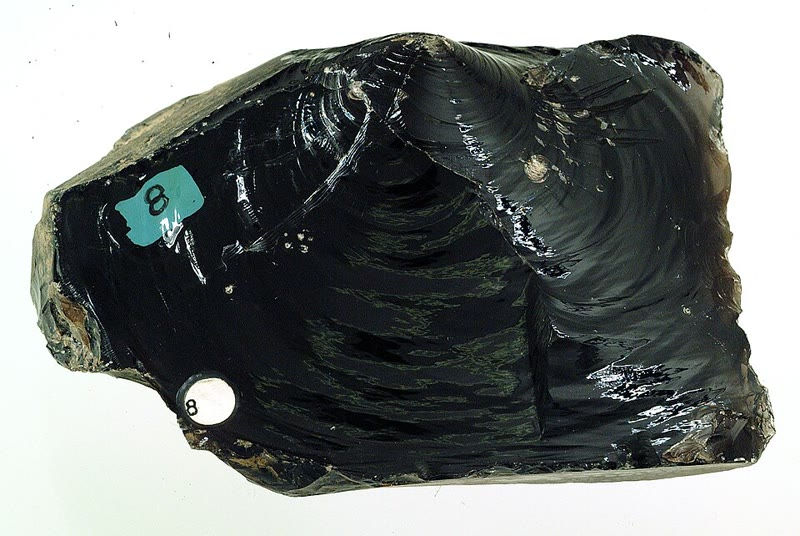
\includegraphics[height=2.75cm]{images/book2/g11-geodil-obsidian.jpg}\hfill
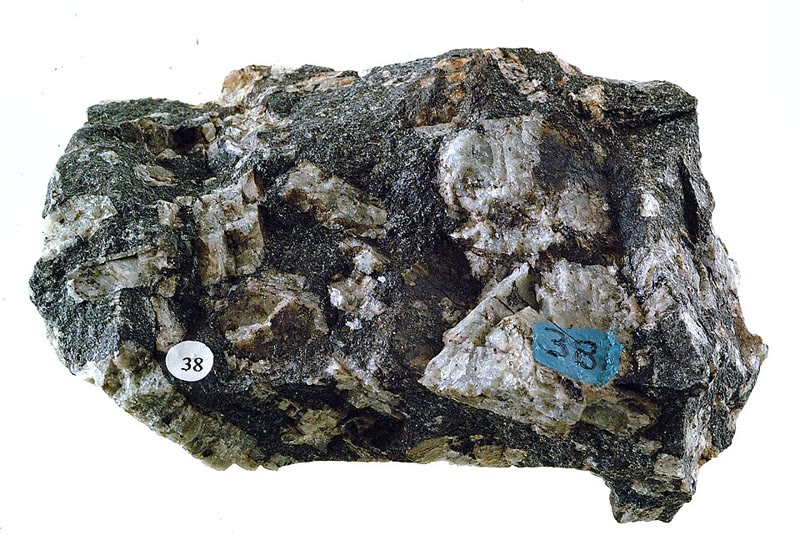
\includegraphics[height=2.75cm]{images/book2/g11-geodil-diabase-porphyry.jpg}\hfill
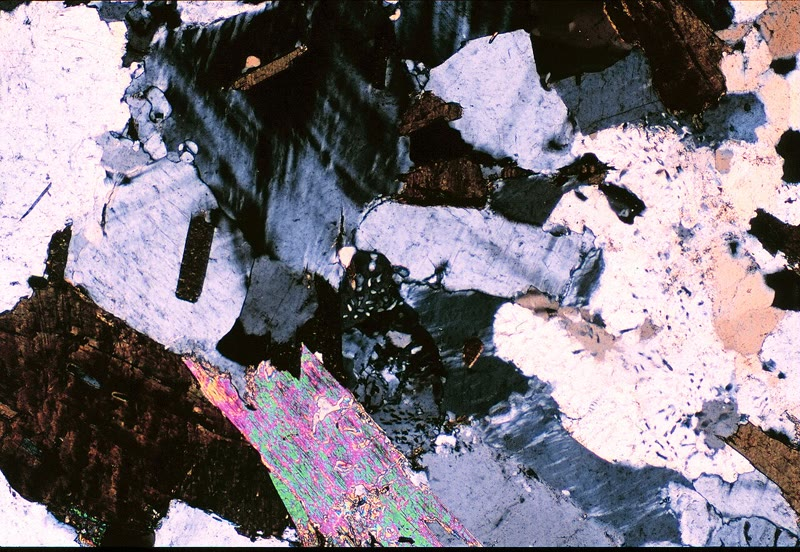
\includegraphics[height=2.75cm]{images/book2/g11-geodil-granite-xpl.jpg}\hfill
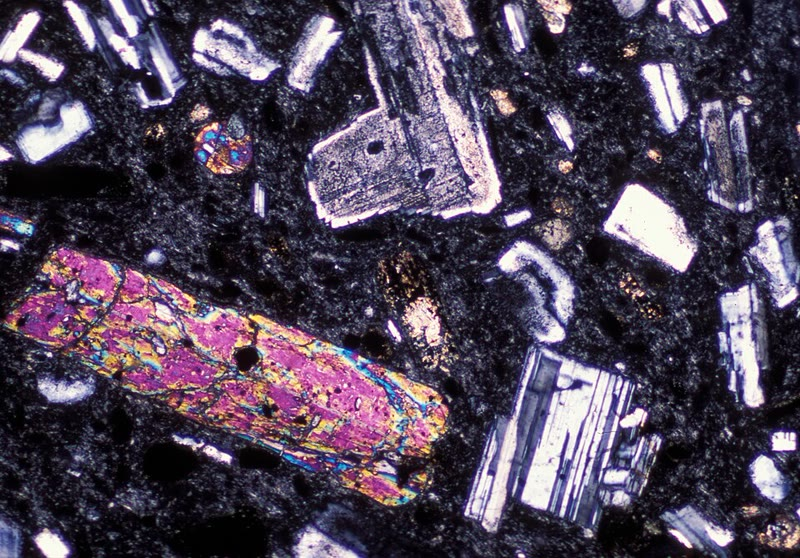
\includegraphics[height=2.75cm]{images/book2/g11-geodil-andesite-xpl.jpg}

{\small Van links naar rechts: obsidiaan, een \omterm{def:g11:igneous-rocks:volcanic-plutonic}{vulkanisch} glas, met zijn gebogen
schelpvormige breuk (\qty{9.5}{cm} breed); een \omterm{def:g11:igneous-rocks:porphyritic}{porfirisch} gesteente, blokvormige
\omterm{def:g11:igneous-rocks:porphyritic}{fenokristen} van plagioklaas in een fijnere grondmassa (\qty{9}{cm}); dan twee
\omterm{def:g11:minerals:thin-section}{slijpplaatjes} tussen gekruiste polarisatoren: een graniet, alle korrels groot en
in elkaar grijpend --- bruin biotiet, een felgekleurde muscoviet, gestreept
plagioklaas, grijs en wit kwarts; een \omterm{def:g11:igneous-rocks:rock-names}{andesiet}, \omterm{def:g11:igneous-rocks:porphyritic}{fenokristen} van
plagioklaas en amfibool in een fijnkorrelige grondmassa. Foto's Twyla
Baker, Mike Davis en Darla Sondrol, Geology Digital Image Library (CC0).}
\end{omfigure}
% ledger: photo:g11-obsidian, photo:g11-diabase-porphyry, photo:g11-granite-xpl, photo:g11-andesite-xpl

\section{Stollingsgesteenten benoemen}

De tweede sleutel tot een stollingsgesteente is zijn chemie, en vooral zijn
gehalte aan silica, \ce{SiO2}, dat in gewone magma's loopt van ongeveer
\qty{45}{\percent} tot ongeveer \qty{75}{\percent} van de massa.

\begin{definition}[Mafisch; intermediair; felsisch]\label{def:g11:igneous-rocks:felsic-mafic}
Een magma, of het gesteente dat het vormt, is \emph{mafisch}\index{mafisch} wanneer het
ongeveer \qty{45}{\percent} tot \qty{55}{\percent} \ce{SiO2} bevat en rijk is aan
ijzer, magnesium en calcium; \emph{intermediair}\index{intermediair (gesteente)}
tussen \qty{55}{\percent} en \qty{65}{\percent}; \emph{felsisch}\index{felsisch}
wanneer het ongeveer \qty{65}{\percent} tot \qty{75}{\percent} \ce{SiO2} bevat en
arm is aan ijzer, magnesium en calcium maar rijk aan natrium en kalium.
\end{definition}
% ledger: tulane:magma-types, earle:magma-oxides

Elk soort magma geeft twee gesteenten, een \omterm{def:g11:igneous-rocks:volcanic-plutonic}{vulkanisch} en fijnkorrelig, een
\omterm{def:g11:igneous-rocks:volcanic-plutonic}{plutonisch} en grofkorrelig, met dezelfde chemie. Basalt en \omterm{def:g11:ocean-ridges:gabbro}{gabbro} zijn
het mafische paar, dat we bij de \omterm{def:g11:ocean-ridges:oceanic-lithosphere}{oceanische korst} zagen; graniet is het felsische plutonische
gesteente. Drie namen maken de reeks compleet.

\begin{definition}[Andesiet; dioriet; ryoliet]\label{def:g11:igneous-rocks:rock-names}
\emph{Andesiet}\index{andesiet} en \emph{dioriet}\index{dioriet} zijn het
vulkanische en het plutonische gesteente van intermediaire samenstelling, vooral opgebouwd uit
plagioklaas met amfibool of pyroxeen. \emph{Ryoliet}\index{ryoliet} is
het vulkanische gesteente van felsische samenstelling, de fijnkorrelige tegenhanger van
graniet.
\end{definition}
% ledger: tulane:magma-types, earle:bowen, photo:g11-andesite, photo:g11-diorite

\begin{omfigure}
\begin{tikzpicture}[font=\footnotesize, x=0.4cm]
  % columns: SiO2 45 to 75 % mapped to x = 45 to 75 (0.4 cm per %)
  \begin{scope}[xshift=-18cm]
  \fill[omLithBasalt!45] (45,0) rectangle (55,2.4);
  \fill[omLithBasalt!20] (55,0) rectangle (65,2.4);
  \fill[omLithGranite!45] (65,0) rectangle (75,2.4);
  \draw[black!60] (45,0) rectangle (75,2.4);
  \draw[black!60] (55,0) -- (55,2.4); \draw[black!60] (65,0) -- (65,2.4);
  \draw[black!60] (45,1.2) -- (75,1.2);
  \foreach \x/\a/\b in {50/basalt/gabbro, 60/andesiet/dioriet, 70/ryoliet/graniet}{
    \node[font=\small\bfseries, text height=1.6ex, text depth=0.3ex] at (\x,1.8) {\a};
    \node[font=\small\bfseries, text height=1.6ex, text depth=0.3ex] at (\x,0.6) {\b};}
  \node[anchor=east, align=right] at (44.4,1.8) {fijnkorrelig\\(vulkanisch)};
  \node[anchor=east, align=right] at (44.4,0.6) {grofkorrelig\\(plutonisch)};
  \node[anchor=south] at (50,2.45) {mafisch};
  \node[anchor=south] at (60,2.45) {intermediair};
  \node[anchor=south] at (70,2.45) {felsisch};
  % minerals (a drawing: where each mineral is common)
  \foreach \y/\a/\b/\m/\c in {-0.55/45.2/52/olivijn/omLithBasalt!80!black,
      -1.15/45.2/61/pyroxeen/omLithBasalt!65!black,
      -1.75/52/69/amfibool/black!60,
      -2.35/57/74.8/biotiet/black!75,
      -2.95/45.2/72/plagioklaas/omDef!45,
      -3.55/63/74.8/kaliveldspaat/omLithGranite!90!red,
      -4.15/64/74.8/kwarts/black!20,
      -4.75/68/74.8/muscoviet/black!35}{
    \fill[\c] (\a,\y) .. controls ({\a+1.2},{\y+0.22}) and ({\b-1.2},{\y+0.22}) .. (\b,\y)
              .. controls ({\b-1.2},{\y-0.22}) and ({\a+1.2},{\y-0.22}) .. (\a,\y) -- cycle;
    \node[anchor=east] at (44.4,\y) {\m};}
  \node[font=\scriptsize, text=black!75] at (50,-2.95) {calciumrijk};
  \node[font=\scriptsize, text=omDef!80!black, anchor=west] at (72.3,-2.95) {natriumrijk};
  % SiO2 axis
  \draw[-{Stealth[length=4pt]}] (45,-5.35) -- (75.8,-5.35);
  \foreach \x in {45,50,...,75} {\draw (\x,-5.35) -- (\x,-5.45); \node[anchor=north] at (\x,-5.45) {\x};}
  \node[anchor=north] at (60,-5.85) {\ce{SiO2} (\unit{\percent} van de massa)};
  \draw[black!30, dashed] (55,0) -- (55,-5.35); \draw[black!30, dashed] (65,0) -- (65,-5.35);
  \end{scope}
\end{tikzpicture}

{\small Gewone stollingsgesteenten benoemen (een tekening). Kolommen: het
silicagehalte van het magma; rijen: fijnkorrelige (vulkanische) en grofkorrelige
(plutonische) gesteenten. Onderaan, waar elk gesteentevormend mineraal veel voorkomt: olivijn
en pyroxeen in mafische gesteenten met calciumrijk plagioklaas; amfibool en
plagioklaas in intermediaire gesteenten; kaliveldspaat, kwarts,
natriumrijk plagioklaas en mica's in felsische gesteenten. De grenzen zijn
geleidelijk.}
\end{omfigure}
% ledger: tulane:magma-types, earle:bowen, earle:magma-oxides, photo:g11-andesite, photo:g11-diorite, photo:g11-granite, nps:granite-minerals

\begin{method}[Een stollingsgesteente benoemen]\label{met:g11:igneous-rocks:naming}
\begin{enumerate}
  \item Bekijk de \omterm{def:g11:igneous-rocks:texture}{textuur}: glasachtig, fijnkorrelig of grofkorrelig;
        \omterm{def:g11:igneous-rocks:porphyritic}{porfirisch} of niet. Fijnkorrelig of glasachtig betekent \omterm{def:g11:igneous-rocks:volcanic-plutonic}{vulkanisch} (of een
        kleine, snel afgekoelde \omterm{def:g11:igneous-rocks:intrusion}{intrusie}); grofkorrelig betekent \omterm{def:g11:igneous-rocks:volcanic-plutonic}{plutonisch}.
  \item Identificeer de mineralen die te zien zijn
        (\cref{met:g11:minerals:identify}): kwarts en kaliveldspaat
        wijzen op \omterm{def:g11:igneous-rocks:felsic-mafic}{felsisch}, amfibool met plagioklaas op \omterm{def:g11:igneous-rocks:felsic-mafic}{intermediair}, olivijn
        en pyroxeen op \omterm{def:g11:igneous-rocks:felsic-mafic}{mafisch}. Gebruik in een fijnkorrelig gesteente de \omterm{def:g11:igneous-rocks:porphyritic}{fenokristen},
        de kleur van de grondmassa --- donker voor \omterm{def:g11:igneous-rocks:felsic-mafic}{mafisch}, licht voor \omterm{def:g11:igneous-rocks:felsic-mafic}{felsisch} ---
        als hint, of een chemische analyse.
  \item Lees de naam af op het kruispunt van de rij en de kolom van het
        schema.
\end{enumerate}
\end{method}

\begin{example}[Twee basalten]
Een donker gesteente uit een lavastroom is overal fijnkorrelig; een ander, van
dezelfde vulkaan, toont groene korrels olivijn van een paar millimeter in een
donkere grondmassa. Beide zijn \omterm{def:g11:igneous-rocks:felsic-mafic}{mafisch} en fijnkorrelig: beide zijn basalten. Het
tweede is een \omterm{def:g11:igneous-rocks:porphyritic}{porfirisch} basalt: zijn olivijn groeide eerst, langzaam, in het
magma onder de vulkaan, voordat de lava uitbarstte en eromheen stolde.
\end{example}
% ledger: photo:g11-olivine, earle:bowen, tulane:textures

\begin{omfigure}
\makebox[0.32\linewidth]{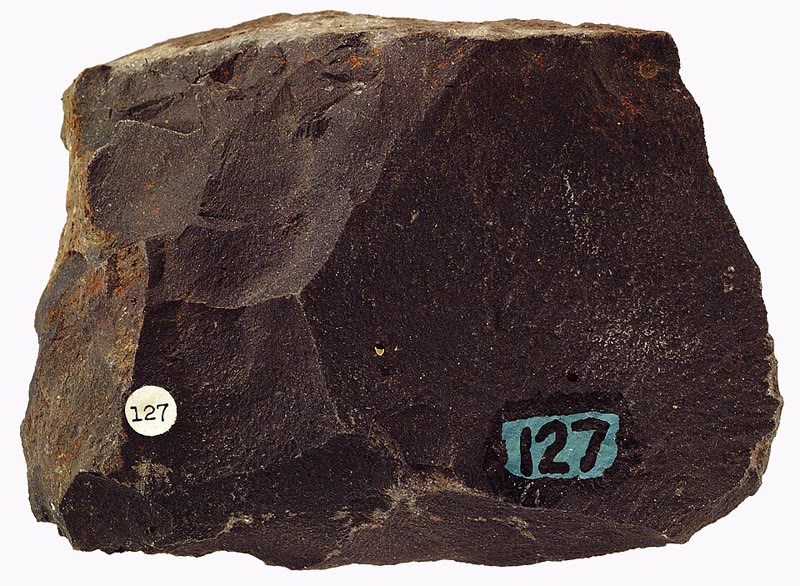
\includegraphics[height=2.9cm]{images/book2/g11-geodil-basalt.jpg}}\hfill
\makebox[0.32\linewidth]{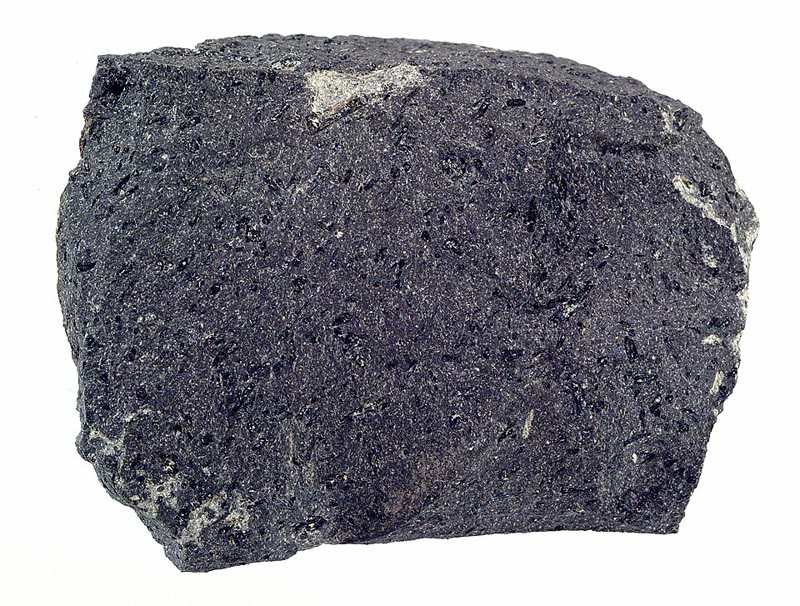
\includegraphics[height=2.9cm]{images/book2/g11-geodil-andesite.jpg}}\hfill
\makebox[0.32\linewidth]{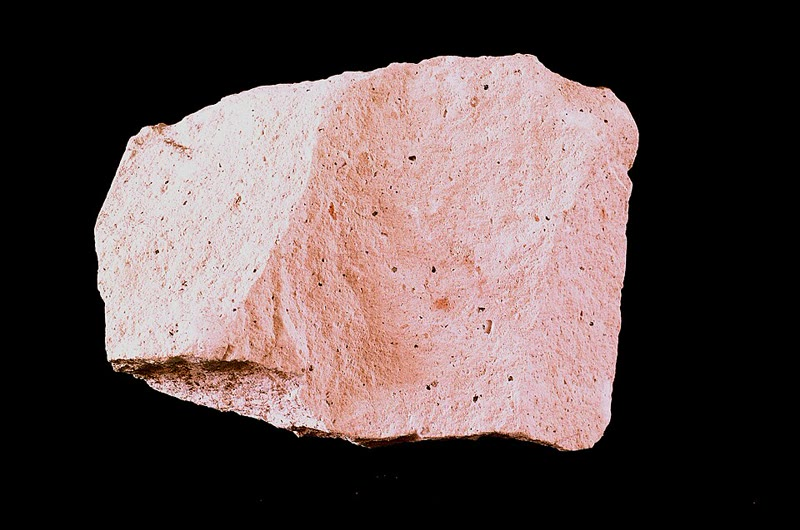
\includegraphics[height=2.9cm]{images/book2/g11-geodil-rhyolite.jpg}}

\smallskip
\makebox[0.32\linewidth]{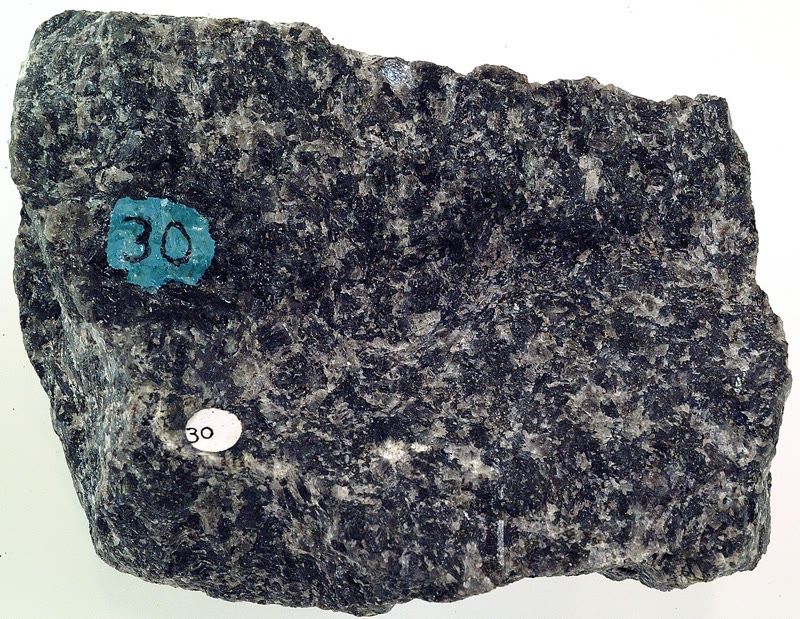
\includegraphics[height=2.9cm]{images/book2/g11-geodil-gabbro.jpg}}\hfill
\makebox[0.32\linewidth]{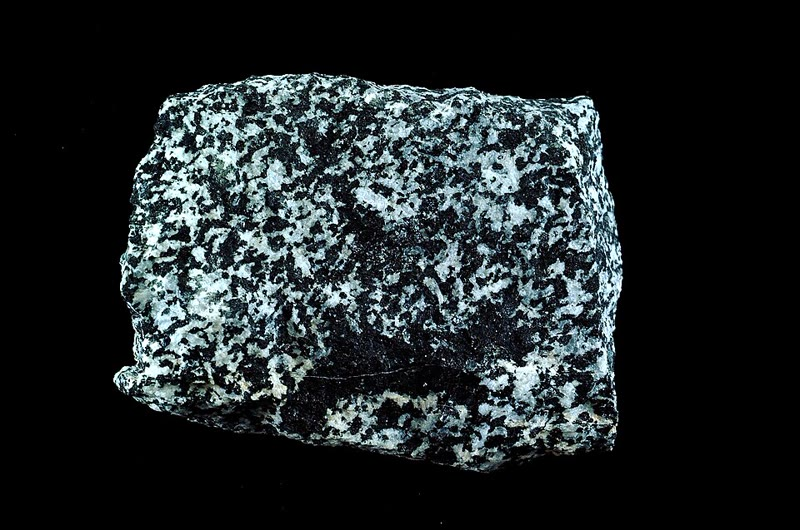
\includegraphics[height=2.9cm]{images/book2/g11-geodil-diorite.jpg}}\hfill
\makebox[0.32\linewidth]{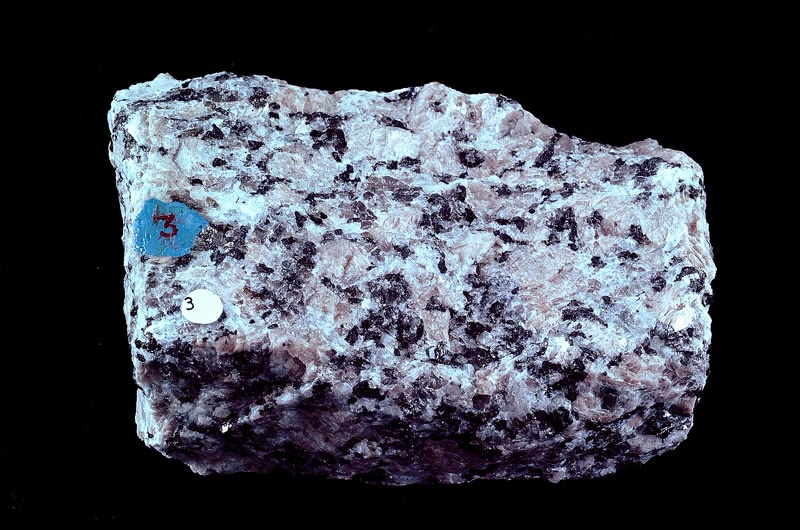
\includegraphics[height=2.9cm]{images/book2/g11-geodil-granite.jpg}}

{\small De drie paren stollingsgesteenten, van \omterm{def:g11:igneous-rocks:felsic-mafic}{mafisch} tot \omterm{def:g11:igneous-rocks:felsic-mafic}{felsisch} van links naar rechts:
\omterm{def:g11:igneous-rocks:volcanic-plutonic}{vulkanisch} boven, \omterm{def:g11:igneous-rocks:volcanic-plutonic}{plutonisch} onder. Boven: een fijnkorrelig basalt; een \omterm{def:g11:igneous-rocks:rock-names}{andesiet}, kleine
amfiboolkristallen in een fijnkorrelige grondmassa (ongeveer \qty{10}{cm});
een roze \omterm{def:g11:igneous-rocks:rock-names}{ryoliet}. Onder: \omterm{def:g11:ocean-ridges:gabbro}{gabbro} (\qty{9}{cm}); \omterm{def:g11:igneous-rocks:rock-names}{dioriet}, zwarte hoornblende en
glazig plagioklaas (\qty{10}{cm}); een grof graniet met grote lichtroze
kaliveldspaten, grijs plagioklaas, kwarts, biotiet en hoornblende
(\qty{10}{cm}). Foto's Nessa Eull, Twyla Baker, Joseph H.~Hartman,
Darla Sondrol en Dexter Perkins, Geology Digital Image Library (CC0).}
\end{omfigure}
% ledger: photo:g11-basalt, photo:g11-andesite, photo:g11-rhyolite, photo:g11-gabbro, photo:g11-diorite, photo:g11-granite

\section{De volgorde van kristallisatie}

Een magma bevriest niet bij één temperatuur, zoals water. Zijn mineralen
verschijnen na elkaar terwijl het afkoelt, elk in zijn eigen temperatuurbereik,
zodat een afkoelend magma kristallen kan bevatten en toch grotendeels vloeibaar kan zijn.

\begin{history}[De experimenten van Bowen]
Norman L.~Bowen (1887--1956) kwam in 1912 bij het Geophysical Laboratory van de
Carnegie Institution in Washington. Hij werkte vooral met basaltische
magma's: hij smolt een gesteente in een oven, liet het langzaam afkoelen tot een gekozen
temperatuur zodat er enkele mineralen ontstonden, en schrikte het dan af, zo
snel dat de overgebleven vloeistof een glas werd. Onder de microscoop lieten de
kristallen zien welke mineralen boven die temperatuur waren ontstaan. Herhaald
bij steeds lagere temperaturen gaf het experiment de volgorde waarin de
mineralen verschijnen. Bowen publiceerde deze volgorde in 1922 als een reactiereeks
en zijn boek \emph{The Evolution of the Igneous Rocks} in 1928.
\end{history}
% ledger: carnegie:bowen, earle:bowen

\begin{omfigure}
\begin{tikzpicture}[font=\footnotesize, box/.style={draw=black!60, rounded corners=2pt, fill=#1, minimum width=3.0cm, minimum height=0.62cm, align=center}]
  \node[box=omLithBasalt!45] (ol) at (0,0) {olivijn};
  \node[box=omLithBasalt!35] (px) at (0,-1.1) {pyroxeen};
  \node[box=black!15] (am) at (0,-2.2) {amfibool};
  \node[box=black!25] (bi) at (0,-3.3) {biotiet};
  \draw[-{Stealth[length=4pt]}, line width=0.8pt] (ol) -- (px);
  \draw[-{Stealth[length=4pt]}, line width=0.8pt] (px) -- (am);
  \draw[-{Stealth[length=4pt]}, line width=0.8pt] (am) -- (bi);
  \node[align=center, anchor=south] at (0,0.45) {\textbf{discontinue tak}\\elk mineraal reageert met de vloeistof\\tot het volgende};
  % continuous branch: a wedge from Ca-rich to Na-rich
  \fill[left color=omDef!55, right color=omDef!12, shading angle=180] (5.0,-0.9) -- (6.6,-0.9) -- (6.6,-3.5) -- (5.0,-3.5) -- cycle;
  \shade[top color=omDef!60, bottom color=omDef!10, draw=black!60, rounded corners=2pt] (4.3,-0.85) rectangle (7.3,-3.55);
  \node[align=center] at (5.8,-1.3) {calciumrijk\\plagioklaas};
  \node[align=center] at (5.8,-3.15) {natriumrijk\\plagioklaas};
  \draw[-{Stealth[length=4pt]}, line width=0.8pt] (5.8,-1.65) -- (5.8,-2.7);
  \node[align=center, anchor=south] at (5.8,0.45) {\textbf{continue tak}\\het plagioklaas verandert\\geleidelijk};
  % last minerals
  \node[box=omLithGranite!45, minimum width=7.6cm] (last) at (2.9,-4.75) {kaliveldspaat, kwarts, (muscoviet)};
  \draw[-{Stealth[length=4pt]}, line width=0.8pt] (bi) -- (bi |- last.north);
  \draw[-{Stealth[length=4pt]}, line width=0.8pt] (5.8,-3.55) -- (5.8,-4.43);
  % temperature arrow
  \draw[-{Stealth[length=5pt]}, line width=1pt, omThm] (-2.6,0.3) -- (-2.6,-4.9);
  \node[anchor=east, align=right, text=omThm] at (-2.75,0.1) {eerst,\\\qtyrange{1200}{1300}{\degreeCelsius}};
  \node[anchor=east, align=right, text=omThm] at (-2.75,-4.7) {laatst, ongeveer\\\qtyrange{750}{800}{\degreeCelsius}};
  \node[anchor=east, align=right, text=omThm] at (-2.75,-2.3) {dalende\\temperatuur};
\end{tikzpicture}

{\small De volgorde waarin mineralen uit een afkoelend magma kristalliseren
(de reactiereeks van Bowen, een tekening). Olivijn ontstaat eerst; plagioklaas begint
ongeveer waar ook pyroxeen begint, eerst rijk aan calcium, dan
steeds rijker aan natrium. Kaliveldspaat, kwarts en soms
muscoviet ontstaan als laatste, uit wat er over is van een silicarijke vloeistof.}
\end{omfigure}
% ledger: earle:bowen

Het woord \emph{reactie} doet ertoe. Olivijn is alleen bij hoge temperatuur
stabiel: wanneer het magma afkoelt, reageren olivijnkristallen met silica in de vloeistof
en veranderen ze in pyroxeen,
\[
  \ce{Mg2SiO4 + SiO2 -> 2 MgSiO3},
\]
enzovoort langs de tak, zolang er silica in de vloeistof blijft. Langs
de andere tak blijven plagioklaaskristallen groeien, maar elke nieuwe laag is
rijker aan natrium dan de vorige: een plagioklaaskristal kan zonair zijn, van een
calciumrijke kern tot een natriumrijke rand, zoals de \omterm{def:g11:igneous-rocks:porphyritic}{fenokristen} van plagioklaas in
het \omterm{def:g11:igneous-rocks:rock-names}{andesiet} hierboven.
% ledger: earle:bowen, photo:g11-andesite-xpl

De reeks verklaart het schema. Een \omterm{def:g11:igneous-rocks:felsic-mafic}{mafisch} magma raakt vroeg door zijn silica heen: het
kristalliseert olivijn, pyroxeen en calciumrijk plagioklaas, en geeft een
\omterm{def:g11:ocean-ridges:gabbro}{gabbro} als het langzaam onder de grond afkoelt, een basalt als het snel aan het
oppervlak afkoelt. Alleen een magma dat rijk is aan silica gaat door tot het einde van de reeks en
vormt kaliveldspaat en kwarts: de mineralen van graniet en \omterm{def:g11:igneous-rocks:rock-names}{ryoliet}.
Hoe een magma onderweg van samenstelling verandert, wanneer zijn eerste kristallen
van de vloeistof worden gescheiden, is het onderwerp van het tweede universitaire jaar.
% ledger: earle:bowen, tulane:bowen

\section{Intrusies}

Magma stijgt op omdat het minder dicht is dan de gesteenten eromheen; het baant zich
een weg in breuken en maakt ze wijder. Veel ervan bereikt nooit het oppervlak:
het kristalliseert in de korst als \omterm{def:g11:igneous-rocks:intrusion}{intrusies}, die pas te zien zijn wanneer
erosie de gesteenten erboven heeft verwijderd.
% ledger: tulane:intrusions

\begin{definition}[Gang; sill; pluton]\label{def:g11:igneous-rocks:intrusion}
Een \emph{intrusie}\index{intrusie} is een lichaam van stollingsgesteente dat
binnenin andere gesteenten is gekristalliseerd. Een \emph{gang}\index{gang} is een plaat
stollingsgesteente die de lagen of structuren van de gesteenten waarin hij is binnengedrongen,
doorsnijdt; een \emph{sill}\index{sill} is een plaat die evenwijdig aan de
lagen ligt, ertussen. Een \emph{pluton}\index{pluton} is een grote intrusie van
willekeurige vorm, op diepte gevormd; veel plutonen samen vormen een
batholiet (\cref{ch:g12:subduction-magmatism}).
\end{definition}
% ledger: tulane:intrusions

\omterm{def:g11:igneous-rocks:intrusion}{Gangen} zijn gewoonlijk minder dan \qty{20}{m} breed en \omterm{def:g11:igneous-rocks:intrusion}{sills} minder dan \qty{50}{m}
dik; een \omterm{def:g11:igneous-rocks:intrusion}{sill} wordt meestal door een \omterm{def:g11:igneous-rocks:intrusion}{gang} gevoed. Ondiepe \omterm{def:g11:igneous-rocks:intrusion}{gangen} en \omterm{def:g11:igneous-rocks:intrusion}{sills} koelen snel af:
ze zijn fijnkorrelig, soms \omterm{def:g11:igneous-rocks:porphyritic}{porfirisch}. Tegen het koude gesteente waarin ze
binnendringen, koelen hun randen het snelst af en zijn ze nog fijner van korrel dan
hun midden: een \emph{afschrikrand}, het teken van een lichaam dat heet was toen
het op zijn plaats kwam. De Sierra Nevada van Californië, waar Yosemite ligt,
is een batholiet: de granietachtige gesteenten waarvan de dichtheid werd gemeten in
\cref{ch:g11:minerals}, komen uit ongeveer tweehonderd van zijn \omterm{def:g11:igneous-rocks:intrusion}{plutonen}.
% ledger: tulane:intrusions, usgs91:sierra, photo:g11-el-capitan

\begin{omfigure}
\begin{tikzpicture}[font=\footnotesize, scale=0.9]
  % layered host rocks
  \fill[omLithSand] (0,0) rectangle (14,-1.0);
  \fill[omLithShale] (0,-1.0) rectangle (14,-2.0);
  \fill[omLithLime] (0,-2.0) rectangle (14,-3.0);
  \fill[omLithSand] (0,-3.0) rectangle (14,-4.0);
  \fill[omLithShale] (0,-4.0) rectangle (14,-6.4);
  \foreach \y in {-1,-2,-3,-4} \draw[black!35] (0,\y) -- (14,\y);
  % pluton
  \fill[omLithGranite, draw=black!60] (2.2,-6.4) .. controls (2.4,-4.6) and (3.6,-4.1) .. (5.5,-4.15)
     .. controls (7.4,-4.2) and (9.0,-4.5) .. (9.6,-6.4) -- cycle;
  % sill between the limestone and the shale, fed by the dyke
  \fill[omLithBasalt, draw=black!60] (7.3,-1.88) -- (12.6,-1.88) .. controls (12.9,-1.9) and (12.9,-2.1) .. (12.6,-2.12) -- (7.3,-2.12) -- cycle;
  % dyke from the pluton to the volcano
  \fill[omLithBasalt, draw=black!60] (7.0,-4.18) -- (7.3,-4.2) -- (7.3,0) -- (7.0,0) -- cycle;
  % a second dyke cutting across the layers, not reaching the surface
  \fill[omLithBasalt, draw=black!60] (3.9,-4.15) -- (4.15,-4.15) -- (2.95,-0.6) -- (2.75,-0.6) -- cycle;
  % volcano and lava flow
  \fill[black!65] (5.75,0) -- (7.15,1.35) -- (8.55,0) -- cycle;
  \fill[omLithBasalt!80!black] (8.4,0) -- (11.6,0) -- (11.6,0.1) .. controls (10.5,0.16) and (9.2,0.22) .. (8.3,0.15) -- cycle;
  \draw[black!70] (0,0) -- (5.75,0); \draw[black!70] (8.55,0) -- (14,0);
  % labels
  \node[anchor=south] at (7.15,1.4) {vulkaan};
  \draw[black!60] (10.5,0.15) -- (11.2,0.8); \node[anchor=south west, inner sep=1pt] at (11.2,0.8) {lavastroom};
  \draw[black!60] (7.3,-0.5) -- (8.3,-0.5); \node[anchor=west, fill=omLithSand, inner sep=1pt] at (8.3,-0.5) {gang (doorsnijdt de lagen)};
  \draw[black!60] (11.0,-2.0) -- (11.0,-2.55); \node[anchor=north, fill=omLithLime, inner sep=1pt] at (11.0,-2.55) {sill (tussen de lagen)};
  \draw[black!60] (3.4,-2.5) -- (1.9,-2.5); \node[anchor=east, fill=omLithLime, inner sep=1pt] at (1.9,-2.5) {gang};
  \node[align=center] at (5.9,-5.5) {pluton};
  \node[anchor=east, fill=omLithShale, inner sep=1pt] at (13.85,-5.3) {gelaagde sedimentaire gesteenten};
\end{tikzpicture}

{\small \omterm{def:g11:igneous-rocks:intrusion}{Intrusies} (een tekening, niet op schaal). Een \omterm{def:g11:igneous-rocks:intrusion}{pluton} kristalliseert op diepte;
\omterm{def:g11:igneous-rocks:intrusion}{gangen} doorsnijden de lagen van de gesteenten erboven, waarvan één een
vulkaan voedt; een \omterm{def:g11:igneous-rocks:intrusion}{sill} spreidt zich tussen twee lagen uit. Alleen erosie van de gesteenten erboven
legt deze lichamen aan het oppervlak bloot.}
\end{omfigure}
% ledger: tulane:intrusions

Hoe lang doet een \omterm{def:g11:igneous-rocks:intrusion}{intrusie} erover om te kristalliseren? Neem een plaat
magma --- een \omterm{def:g11:igneous-rocks:intrusion}{gang} of een \omterm{def:g11:igneous-rocks:intrusion}{sill} --- met dikte $b$, die haar warmte door
geleiding verliest aan het gesteente aan beide kanten. De enige grootheden die het
tempo bepalen, zijn de dikte $b$, in meter, en de thermische diffusiviteit $\kappa$,
in \unit{m^2/s}; de enige tijd die je ermee kunt bouwen, is $b^2/\kappa$.
% ledger: england:kelvin, delaney86:example

\begin{proposition}[De afkoelingstijd van een plaat magma]\label{prop:g11:igneous-rocks:cooling}
Een plaat magma met dikte $b$ die door geleiding afkoelt, stolt in een
tijd
\[
  t = C\,\frac{b^2}{\kappa},
\]
waarbij $\kappa$ de thermische diffusiviteit van de gesteenten is en $C$ een getal dat wordt bepaald
door de temperaturen van het magma en van het omringende gesteente en door de warmte
die vrijkomt wanneer het magma kristalliseert. Een verdubbeling van de dikte vermenigvuldigt de
tijd met vier. (Aangenomen; de waarde van $C$ komt uit een berekend model.)
\end{proposition}
% ledger: delaney86:properties, delaney86:example

Voor een basaltisch magma dat bij \qty{1150}{\degreeCelsius} binnendringt in gesteente van
\qty{50}{\degreeCelsius}, dat volledig kristalliseert bij
\qty{950}{\degreeCelsius} en \qty{900}{MJ} warmte vrijgeeft per kubieke
meter die kristalliseert, met $\kappa = \qty{1e-6}{m^2/s}$, geeft het model
$C \approx 0.21$. Een plaat van \qty{2}{m} dik stolt dan in ongeveer tien
dagen, een \omterm{def:g11:igneous-rocks:intrusion}{sill} van \qty{20}{m} dik in ongeveer tweeënhalf jaar, een van
\qty{100}{m} dik in ongeveer vijfenzestig jaar. Zonder de kristallisatiewarmte
zouden de tijden drie keer korter zijn: kristalliserend
magma houdt zichzelf warm.
% values (dyke_cooling.py): t2_day 9.55, t20_yr 2.61, t100_yr 65.3, latent_factor 2.94; C = 8.2475e7 s / 4e8 s = 0.206
% ledger: delaney86:example, delaney86:properties, england:kelvin

\begin{omfigure}
\begin{tikzpicture}
\begin{axis}[omrecord, name=times, width=0.45\linewidth, height=5.0cm, xmode=log, ymode=log,
  xmin=0.8, xmax=130, ymin=1e-3, ymax=200, xlabel={dikte van de plaat (\unit{m})},
  ylabel={tijd tot stollen (jaar)},
  legend style={font=\scriptsize, at={(0.5,-0.4)}, anchor=north, legend columns=2,
    /tikz/every even column/.append style={column sep=4pt}}]
% computed in figdata/grade-11/dyke_cooling.py; ledger: delaney86:*, england:kelvin
\addplot[omThm, line width=1pt, mark=*, mark size=1.4pt] table[x=b, y=t_yr] {figdata/out/grade-11-dyke_cooling-times.dat};
\addplot[omDef, line width=1pt, dashed, mark=o, mark size=1.4pt] table[x=b, y=t0_yr] {figdata/out/grade-11-dyke_cooling-times.dat};
\legend{met kristallisatiewarmte, zonder}
\end{axis}
\begin{axis}[omrecord, at={(times.east)}, anchor=west, xshift=1.6cm, width=0.45\linewidth, height=5.0cm,
  xmin=-28, xmax=28, ymin=0, ymax=1300, xlabel={afstand tot het midden van de sill (\unit{m})},
  ylabel={temperatuur (\unit{\degreeCelsius})},
  legend style={font=\scriptsize, at={(0.5,-0.4)}, anchor=north, legend columns=4,
    /tikz/every even column/.append style={column sep=4pt}}]
\fill[omLithBasalt!30] (axis cs:-10,0) rectangle (axis cs:10,1300);
\draw[black!50, dashed] (axis cs:-28,950) -- (axis cs:28,950);
\node[font=\scriptsize, anchor=south east, text=black!60] at (axis cs:27,955) {solidus};
\node[font=\scriptsize, anchor=north] at (axis cs:0,1290) {sill};
% computed in figdata/grade-11/dyke_cooling.py
\addplot[omProp, line width=0.9pt] table[x=x, y=T1] {figdata/out/grade-11-dyke_cooling-profiles.dat};
\addplot[omThm, line width=0.9pt] table[x=x, y=T2] {figdata/out/grade-11-dyke_cooling-profiles.dat};
\addplot[omDef, line width=0.9pt] table[x=x, y=T3] {figdata/out/grade-11-dyke_cooling-profiles.dat};
\addplot[black, line width=0.9pt] table[x=x, y=T4] {figdata/out/grade-11-dyke_cooling-profiles.dat};
\legend{30 dagen, 6 maanden, 1 jaar, 2 jaar}
\end{axis}
\end{tikzpicture}

{\small Een plaat basaltisch magma die door geleiding afkoelt (berekend model).
Links: de tijd die ze nodig heeft om te stollen, tegen haar dikte, op logaritmische
assen: een rechte lijn met helling 2, waarbij de tijd groeit als het kwadraat van de
dikte. Rechts: temperaturen dwars door een \omterm{def:g11:igneous-rocks:intrusion}{sill} van \qty{20}{m} dik (gearceerd),
binnengedrongen bij \qty{1150}{\degreeCelsius} in gesteente van
\qty{50}{\degreeCelsius}. De randen zakken meteen onder de solidus, het
midden pas na ongeveer tweeënhalf jaar.}
\end{omfigure}
% values (dyke_cooling.py): profiles at 30, 180, 365, 730 days; contact about 690 degC (Delaney: 690)

Het model laat ook zien hoe de afschrikrand ontstaat. Het gesteente bij het contact
springt meteen naar ongeveer \qty{690}{\degreeCelsius}, ver onder de solidus: de
eerste centimeters van de \omterm{def:g11:igneous-rocks:intrusion}{sill} bevriezen binnen een dag, terwijl het midden jarenlang
vloeibaar blijft. Echte \omterm{def:g11:igneous-rocks:intrusion}{intrusies} zijn ingewikkelder --- de eigenschappen van
gesteenten veranderen met de temperatuur, water circuleert, een diepe \omterm{def:g11:igneous-rocks:intrusion}{pluton} zit in gesteente
dat al heet is en kan keer op keer opnieuw worden gevoed --- en daarom hebben grote
diepe \omterm{def:g11:igneous-rocks:intrusion}{intrusies} veel langer nodig om af te koelen dan de wet, met een koud omringend gesteente,
zou doen vermoeden.
% ledger: delaney86:example, tulane:cooling-times
% values (dyke_cooling.py): margin_day_20m 0.58 (cell 12.5 cm from the contact)

\section{Oefeningen}

\begin{exercise}[$\star$]\label{exo:g11:igneous-rocks:1}
Definieer een \omterm{def:g11:igneous-rocks:volcanic-plutonic}{vulkanisch gesteente} en een \omterm{def:g11:igneous-rocks:volcanic-plutonic}{plutonisch gesteente}. Geef de drie paren
vulkanische en plutonische gesteenten van dezelfde samenstelling, van \omterm{def:g11:igneous-rocks:felsic-mafic}{mafisch} tot \omterm{def:g11:igneous-rocks:felsic-mafic}{felsisch}.
\end{exercise}

\begin{exercise}[$\star$]\label{exo:g11:igneous-rocks:2}
Koppel elk gesteente aan zijn \omterm{def:g11:igneous-rocks:texture}{textuur} --- glasachtig, fijnkorrelig, grofkorrelig,
\omterm{def:g11:igneous-rocks:porphyritic}{porfirisch}: (1) obsidiaan; (2) graniet; (3) een basalt met groene olivijnkristallen
van een paar millimeter in een donkere grondmassa; (4) een basalt waarin
geen mineraal te zien is.
\end{exercise}

\begin{exercise}[$\star$]\label{exo:g11:igneous-rocks:3}
Drie magma's bevatten \qty{48}{\percent}, \qty{60}{\percent} en
\qty{72}{\percent} \ce{SiO2}. Classificeer elk, en noem het gesteente dat elk geeft
wanneer het langzaam op diepte afkoelt.
\end{exercise}

\begin{exercise}[$\star$]\label{exo:g11:igneous-rocks:4}
Definieer een \omterm{def:g11:igneous-rocks:intrusion}{gang}, een \omterm{def:g11:igneous-rocks:intrusion}{sill} en een \omterm{def:g11:igneous-rocks:intrusion}{pluton}. Welk lichaam voedde de vulkaan op de
tekening van \omterm{def:g11:igneous-rocks:intrusion}{intrusies} in dit hoofdstuk?
\end{exercise}

\begin{exercise}[$\star$]\label{exo:g11:igneous-rocks:5}
Welk mineraal ontstaat in de reactiereeks van Bowen als eerste, en welke mineralen
als laatste? Hoe verandert plagioklaas terwijl het magma afkoelt?
\end{exercise}

\begin{exercise}[$\star\star$]\label{exo:g11:igneous-rocks:6}
Twee gesteenten worden geanalyseerd (massapercentages). Gesteente A: \ce{SiO2} 74, \ce{Al2O3}
14, \ce{FeO} 3, \ce{CaO} 3, \ce{MgO} 0.5, \ce{Na2O} 5, \ce{K2O} 4. Gesteente B:
\ce{SiO2} 47, \ce{Al2O3} 14, \ce{FeO} 8, \ce{CaO} 10, \ce{MgO} 8, \ce{Na2O}
1, \ce{K2O} 2. (1) Classificeer elk. (2) Controleer je antwoord met de andere
oxiden. (3) Gesteente A is fijnkorrelig: benoem het. Gesteente B is grofkorrelig: benoem
het.
\end{exercise}

\begin{exercise}[$\star\star$]\label{exo:g11:igneous-rocks:7}
Een \omterm{def:g11:igneous-rocks:intrusion}{gang} van \qty{2}{m} dik stolt in ongeveer tien dagen. Hoe lang doet een \omterm{def:g11:igneous-rocks:intrusion}{gang} van
hetzelfde magma erover, volgens de propositie over de afkoelingstijd, als hij
\qty{1}{m} dik is? Een \omterm{def:g11:igneous-rocks:intrusion}{sill} van \qty{20}{m} dik? Een van \qty{200}{m} dik?
\end{exercise}

\begin{exercise}[$\star\star$]\label{exo:g11:igneous-rocks:8}
(1) Toon aan dat $b^2/\kappa$ een tijd is. (2) Bereken die voor $b = \qty{20}{m}$
en $\kappa = \qty{1e-6}{m^2/s}$, in seconden en in jaren
($\num{1}\text{ jaar} \approx \qty{3.16e7}{s}$). (3) Hoe lang doet de \omterm{def:g11:igneous-rocks:intrusion}{sill} er met $C = 0.21$
over om te stollen?
\end{exercise}

\begin{exercise}[$\star\star$]\label{exo:g11:igneous-rocks:9}
Een gesteente toont blokvormige plagioklaaskristallen van ongeveer een centimeter lang in een
grondmassa waarvan de korrels niet te zien zijn. Beschrijf zijn \omterm{def:g11:igneous-rocks:texture}{textuur}, en vertel het
verhaal van zijn afkoeling in twee fasen.
\end{exercise}

\begin{exercise}[$\star\star$]\label{exo:g11:igneous-rocks:10}
Olivijn reageert met silica in de vloeistof: $\ce{Mg2SiO4 + SiO2 -> 2
MgSiO3}$. (1) Controleer dat de vergelijking klopt. (2) Welke massa silica neemt
\qty{1}{kg} olivijn uit de vloeistof op, met de molaire massa's
\qty{140.7}{g/mol} (\ce{Mg2SiO4}) en \qty{60.1}{g/mol} (\ce{SiO2})? (3) Waarom
behoudt een magma dat arm is aan silica zijn olivijn?
\end{exercise}

\begin{exercise}[$\star\star$]\label{exo:g11:igneous-rocks:11}
Een \omterm{def:g11:igneous-rocks:intrusion}{sill} van \qty{20}{m} dik en \qty{1}{m^2} oppervlakte koelt af van
\qty{1150}{\degreeCelsius} tot \qty{50}{\degreeCelsius}. (1) Zijn
warmtecapaciteit is \qty{2.5}{MJ} per kubieke meter en per graad: hoeveel warmte
verliest hij door af te koelen? (2) Hij geeft ook \qty{900}{MJ} per kubieke meter vrij terwijl hij
kristalliseert: hoeveel warmte is dat? (3) Vergelijk de twee.
\end{exercise}

\begin{exercise}[$\star\star\star$]\label{exo:g11:igneous-rocks:12}
In het berekende model van een \omterm{def:g11:igneous-rocks:intrusion}{sill} van \qty{20}{m} dik zakt het gesteente op
\qty{12.5}{cm} van het contact na ongeveer \num{0.6}~dag onder de solidus,
het gesteente op \qty{5}{m} van het contact na ongeveer 545 dagen,
en het midden na ongeveer 950 dagen. (1) Waar in de \omterm{def:g11:igneous-rocks:intrusion}{sill} verwacht je de
kleinste kristallen, en waar de grootste? (2) Is de snelheid waarmee de
vaste laag groeit constant? (3) Waarom is de \omterm{def:g11:igneous-rocks:intrusion}{sill} zelfs in zijn
midden fijnkorrelig, vergeleken met een graniet?
\end{exercise}

\begin{exercise}[$\star\star\star$]\label{exo:g11:igneous-rocks:13}
Een \omterm{def:g11:igneous-rocks:intrusion}{pluton} is \qty{2}{km} dik. (1) Schat zijn afkoelingstijd met de propositie en de
\omterm{def:g11:igneous-rocks:intrusion}{sill} van \qty{20}{m} (ongeveer 2.6 jaar). (2) Van grote
diepe \omterm{def:g11:igneous-rocks:intrusion}{intrusies} is bekend dat ze tot miljoenen jaren nodig hebben om af te koelen. Geef twee
redenen waarom de eenvoudige wet de tijd onderschat.
\end{exercise}

\begin{exercise}[$\star\star\star$]\label{exo:g11:igneous-rocks:14}
Felsische magma's barsten uit bij ongeveer \qtyrange{650}{800}{\degreeCelsius}, mafische
magma's bij ongeveer \qtyrange{1000}{1200}{\degreeCelsius}. Leg met de
reactiereeks van Bowen uit waarom een graniet kaliveldspaat, kwarts
en natriumrijk plagioklaas bevat, en geen olivijn, terwijl een \omterm{def:g11:ocean-ridges:gabbro}{gabbro} olivijn,
pyroxeen en calciumrijk plagioklaas bevat, en geen kwarts.
\end{exercise}

\begin{exercise}[$\star\star\star$]\label{exo:g11:igneous-rocks:15}
Materiaal dat in de lucht wordt uitgeworpen, koelt in seconden af, lavastromen in dagen tot weken,
ondiepe \omterm{def:g11:igneous-rocks:intrusion}{intrusies} in maanden tot jaren. (1) Welke dikte van een plaat stolt
volgens de propositie in ongeveer een dag? (2) Een lavastroom van \qty{5}{m}
dik stolt in ongeveer een maand: klopt dat met de wet voor een
plaat die aan beide kanten afkoelt? (3) Welke \omterm{def:g11:igneous-rocks:texture}{textuur} verwacht je in elk geval?
\end{exercise}

\section{Probleem: een sill en zijn kristallen}

\begin{problem}[{Weekendprobleem --- hoe lang een sill erover doet om te bevriezen}]
\label{pb:g11:igneous-rocks:1}
% values (dyke_cooling.py): t20_yr 2.61, margin_day_20m 0.58, t2_day 9.55, contact ~690 degC;
% C = 0.206; ledger delaney86:*, tulane:*, earle:*
In de wand van een dal ligt een donkere plaat stollingsgesteente van \qty{20}{m} dik
tussen twee zandsteenlagen, evenwijdig eraan. Er worden monsters genomen van
de rand tot het midden. Bij het contact is het gesteente heel fijnkorrelig, bijna
glasachtig; \qty{1}{m} naar binnen zijn de kristallen ongeveer \qty{0.1}{mm}; in het
midden ongeveer \qty{1}{mm}, en zijn plagioklaas en pyroxeen met een loep net uit elkaar
te houden.

\medskip
\noindent\textbf{Deel I --- De texturen.}
\begin{enumerate}
  \item Is de plaat een \omterm{def:g11:igneous-rocks:intrusion}{gang} of een \omterm{def:g11:igneous-rocks:intrusion}{sill}? Waarom?
  \item Beschrijf de \omterm{def:g11:igneous-rocks:texture}{textuur} bij het contact en in het midden.
  \item Waarom is het gesteente bij het contact het fijnst van korrel?
  \item Hoe heet deze fijnkorrelige rand, en wat bewijst hij over
        de temperatuur van de plaat toen die op haar plaats kwam?
  \item De plaat wordt van onderen gevoed door een verticale plaat van hetzelfde gesteente,
        \qty{2}{m} dik, die de zandsteen doorsnijdt. Wat is dat?
\end{enumerate}

\medskip
\noindent\textbf{Deel II --- Het gesteente benoemen.}
\begin{enumerate}[resume]
  \item Een analyse geeft \qty{49}{\percent} \ce{SiO2}, \qty{10}{\percent}
        \ce{FeO}, \qty{7}{\percent} \ce{MgO} en \qty{10}{\percent}
        \ce{CaO}. Is het magma \omterm{def:g11:igneous-rocks:felsic-mafic}{mafisch}, \omterm{def:g11:igneous-rocks:felsic-mafic}{intermediair} of \omterm{def:g11:igneous-rocks:felsic-mafic}{felsisch}?
  \item Welke mineralen verwacht je volgens de reeks van Bowen?
  \item Welke naam past bij het gesteente van het contact? Welk \omterm{def:g11:igneous-rocks:volcanic-plutonic}{plutonisch gesteente} heeft
        dezelfde samenstelling?
  \item Waarom kan één lichaam magma gesteenten met verschillende texturen geven?
  \item In welke volgorde begonnen olivijn, pyroxeen en plagioklaas te
        kristalliseren?
\end{enumerate}

\medskip
\noindent\textbf{Deel III --- De afkoelingstijd.}
\begin{enumerate}[resume]
  \item Bereken $b^2/\kappa$ voor de \omterm{def:g11:igneous-rocks:intrusion}{sill}, met $\kappa = \qty{1e-6}{m^2/s}$,
        in seconden.
  \item Het model geeft $C = 0.206$. Bereken de tijd die de \omterm{def:g11:igneous-rocks:intrusion}{sill} nodig had om te stollen, in
        seconden, dan in jaren ($\num{1}\text{ jaar} \approx \qty{3.16e7}{s}$).
  \item Hoe lang deed de voedende plaat, \qty{2}{m} dik, erover?
  \item Zonder de kristallisatiewarmte zou $C$ ongeveer $0.07$ zijn.
        Hoe lang zou de \omterm{def:g11:igneous-rocks:intrusion}{sill} er dan over doen? Waarom vertraagt kristallisatie de
        afkoeling?
  \item Het model geeft ongeveer \num{0.6}~dag voor het gesteente op \qty{12.5}{cm}
        van het contact. Hoeveel keer sneller bevroor het dan het
        midden?
\end{enumerate}

\medskip
\noindent\textbf{Deel IV --- Wat de kristallen vertellen.}
\begin{enumerate}[resume]
  \item Lavastromen koelen in dagen tot weken af, ondiepe \omterm{def:g11:igneous-rocks:intrusion}{intrusies} in maanden tot
        jaren. Waar past de \omterm{def:g11:igneous-rocks:intrusion}{sill}?
  \item Een graniet met kristallen van een centimeter of meer koelde veel
        langzamer af. Schat met de wet de dikte van een plaat die
        duizend keer langer nodig zou hebben dan de \omterm{def:g11:igneous-rocks:intrusion}{sill}.
  \item Waarom moet zo'n lichaam diep in de korst zijn ontstaan?
  \item De \omterm{def:g11:igneous-rocks:intrusion}{sill} is vandaag aan het oppervlak te zien. Wat moet er gebeurd zijn met
        de gesteenten die erboven lagen?
  \item Besluit: hoe lang deed de \omterm{def:g11:igneous-rocks:intrusion}{sill} erover om te stollen?
\end{enumerate}
\end{problem}
